% !TEX root = ../my-thesis.tex
%
\chapter{Theoretical Foundations}
\label{sec:theory}
Before presenting the approach for tackling AutoML with an ensemble of optimizers, some theoretical foundations of both elements, AutoML and optimization, are given in the following.
This theoretical background is structured in three parts:
\begin{enumerate}
    \item Some basic concepts and intuitions of machine learning in general are outlined alongside with the challenges and problems that arise when applying machine learning.
    \item The concepts and usual approaches of AutoML are introduced, which were developed to tackle the listed challenges of classical machine learning. In addition, the connection between the AutoML setting and typical optimization problems is illustrated.
    \item As the foundation for building an ensemble of optimizers a selection of established optimization methods is given and explained.
\end{enumerate}
The overview of optimization methods is concluded with the discussion of a theoretical drawback of using a single optimization method.
This discussion of a possible disadvantage is used as a starting point for the line of reasoning why an ensemble of optimizers is an approach to counteract this drawback.
Before explaining the ensemble approach in the next chapter, this line of reasoning is continued with a selection of related works, where other approaches that addressed this theoretical disadvantage of using a single optimization method are mentioned. 

\section{Classical Machine Learning}
\label{sec:theory:ml}
If a human is given a task where the correct solution or reaction is not evident, a humans has always the possibility to react with a random solution or with an arbitrary reaction.
But if the human has any prior first- or second-hand experience with the same of a similar task, the human can choose the reaction based on the memories of different outcomes for different reactions for the more or less similar prior task.
With the high abstraction level and very symbolic nature of human thinking and memorization, it is comparably easy for humans to recognize even remote similarities between tasks.\newline
This is very challenging for a computer in contrast, because the models of tasks, experiences, and outcomes of reactions to tasks have to be readable and understandable for a machine, i.e. be in any kind of structured and consistent format.
This setting can be formalized as a combination of $T, P$ and $E$, where $T$ is a class of tasks, $P$ a performance measurement for solutions of a specific instances of the tasks class $T$ and $E$ is either given or collected experience, i.e. performance measurements for certain solutions in the context of specific task instance $t\in T$~\cite{Mitchell-MachineLearning}.\newline
Of course it is possible for a human programmer to manually specify the solution with the best performance measurement for any possible $t\in T$ but for a high $|T|$ this is rarely possible and viable.
Here, machine learning has its use-case: "Machine learning enables us to tackle tasks that are too difficult to solve with fixed programs written and designed by human beings"~\cite{Goodfellow-DeepLearning}.\newline
A high number of different types of task classes $T$ is imaginable, but one of the common one is \textit{Supervised Learning}.
In supervised learning, $T$ includes a fix set of all possible solutions $S$.
The concrete task for Supervised Learning is now to select for a given $t\in T$ a $s\subseteq S$ such that $P(t,s)$ is optimal.
To enable a machine to learn supervised, the experience $E$ has to be successively build in the form of $\{(t_1, s_1, P(t_1, s_1)), ..., (t_n, s_n, P(t_n s_n))\}$.
For a new task instance $t_i$, the computer will select a $s_i$ based on a decision model build from $E$, receive a performance feedback $P(t_i, s_i)$ and finally enrich $E$ with $(t_i, s_i, P(t_i, s_i))$ as well as updating the decision model with the changed $E$.
Therewith, a well working machine learning algorithm for supervised learning would now be able to achieve $P(t_j, s_j) \geq P(t_i, s_i)$ if $t_j$ and $t_i$ are similar instances, since it already has experience which $s\subseteq S$ had a certain performance value for $t_i$ and might therefore be a good or bad choice for $t_j$.\newline
This task of comparing and judging the similarity of different instances of $T$ and to build a practicable decision model based on $E$ to select a solution out of $S$ has been tackled with a plethora of different algorithms or even combinations of multiple algorithms as a form of machine learning pipeline.
Usually, this algorithms have to be configured with a set of hyperparameter depending on $T$ and often $T$ also has to be transformed before presenting concrete instances to the algorithm for learning, i.e. pre-processing each $t\in T$ with one or more transformation methods.
Without making suitable choices for the machine learning algorithm as well as corresponding hyperparameter and pre-processing methods for each different $T$, the performance measurements will only increase for a high $|E|$ or even not at all.
But because the number of available task instances, i.e. the amount of data, that can be used to build $E$ with a machine learning algorithm is often limited for most use-case domains, a valid choice for the learning algorithm, hyperparameter and, if necessary, pre-processing methods is crucial.\newline
With the high number of available machine learning algorithms and the often complex relationships between learning performance and hyperparameter configurations of the chosen algorithm as well as properties of $T$ and suitable pre-processing methods a big expertise in the machine learning field is necessary to be able to assemble machine learning applications with good performance measurements.
Since this necessary expertise in machine learning is not broadly available and a lot of companies or research facilities have a high demand for machine learning applications, it is not possible to apply machine learning in every use-case where it might be beneficial.
This accelerated the emergence of the machine learning research sub-topic \textit{Automated Machine Learning}. 

\section{Automated Machine Learning}
\label{sec:theory:automl}
Automated Machine Learning, or short \textit{AutoML}, tries to tackle this knowledge barrier, which prevents interested people from applying machine learning.
Therefore, the overall goal is to automate most tasks of the process of creating a machine learning application that would require machine learning knowledge.\newline
In this chapter at first a description of the general workflow of an AutoML tool is given and the usual two main steps of this workflow are illustrated.
This will be concluded with an formalization of the AutoML problem setting as an optimization problem.

\subsection{General Workflow}
\label{sec:theory:automl:workflow}
AutoML application are usually designed very homogeneous and therefore have very similar workflows among themselves.
As an input, the application will receive data in an machine-readable format and usually some form of constraint for its execution.
The expected outputs are the performance of the found machine learning pipeline regarding some task-dependent metric and the best found machine learning pipeline for the given data itself.
Additionally, each AutoML tool can have further configuration necessary as an input.\newline
The constraints for execution are required to prevent the AutoML tool from searching for the best machine learning pipeline for the given data indefinitely with probably continuously growing hardware consumption.
Therefore, the time and/or some hardware budgets are constrained.
This inputs and outputs of an conceptual AutoML tool are illustrated in figure~\ref{fig:theory:conceptualAutoMLTool}.\newline
\begin{figure}[ht!]
    \centering
    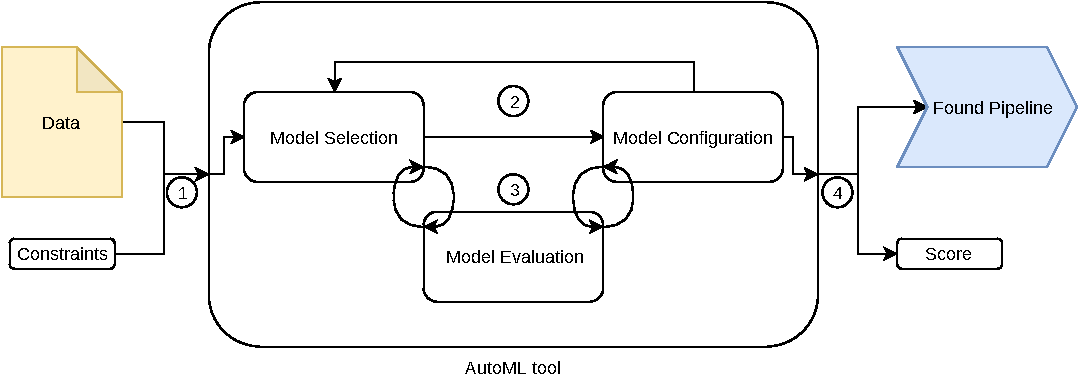
\includegraphics[width=\textwidth]{gfx/Figures/Theory/AutoMLTool.pdf}
    \caption{High level view of a conceptual AutoML tool. }
	\label{fig:theory:conceptualAutoMLTool}
\end{figure}
The general workflow of an AutoML tool is also numbered and illustrated in the figure and can be generalized with the following steps:
\begin{enumerate}
    \item AutoML tool gets input data and some execution constraints as an input.
    \item Model Selection and Model Configuration are repeated until execution constraints are met.
    \item Model Selection as well as Model Configuration can perform a Model Evaluation to get a score for any pipeline candidate they encounter.
    \item After the constraints are met, the best found pipeline as well as the score of this pipeline are given as an output.
\end{enumerate}
The Model Evaluation step is usually performed by training a pipeline on one big portion of the input data and testing it with a smaller portion of the data, sometimes called validation data, while measuring some kind of performance measurement, for example the accuracy of predictions or some error metric.
But other evaluation techniques for example like a Cross-Validation are also common.\newline
While the Model Evaluation step is only very loosely defined and usually not a complex procedure, the Model Selection and Model Configuration steps of the AutoML workflow are more sophisticated.
They have to select a suitable candidate from a usually large space. 
Both spaces, for Model Selection as well as for Model Configuration, will be individually explained in the following.

\subsection{Model Selection}
\label{sec:theory:automl:selection}
Model Selection is the task of selecting $1$ to $n$ components that will be part of the machine learning pipeline and sequentially traversed when data is passed through the pipeline.
For example, a valid pipeline would be to apply a Principal-Component-Analysis on the data as a first component and to use a Support Vector Machine for classification on the processed data as a second component afterwards.
In this step of the workflow, the space one candidate has to be selected from, consists of all this valid pipeline, which usually have two or more components.\newline
Usually there are three types of components:
\begin{itemize}
    \item Pre-Processing: Transform the input data before presenting it to the learning model.
    \item Learning Model: Perform the actual machine learning task on the data, for example classify a datapoint after training.
    \item Post-Processing: Transform the output of the learning model before yielding it as a final result.
\end{itemize}
Although in theory only a single learning model is necessary and components for pre- and post-processing are optional, at least pre-processing is very common in machine learning pipelines and included most of the time.\newline
It is possible to use more than one component from each type in a single pipeline and pipelines with arbitrary complexity can be created.
More than one pre- or post-processor can be used in sequence or in parallel with some kind of aggregator subsequently.
Equally, more than one learning model can be combined to be used as a composite model with a proper aggregation method like for example Bagging of models~\cite{Breiman-BaggingPredictors}.
An example for such a more complex pipeline is illustrated in figure~\ref{fig:theory:complexPipeline}.\newline
\begin{figure}[ht!]
    \centering
    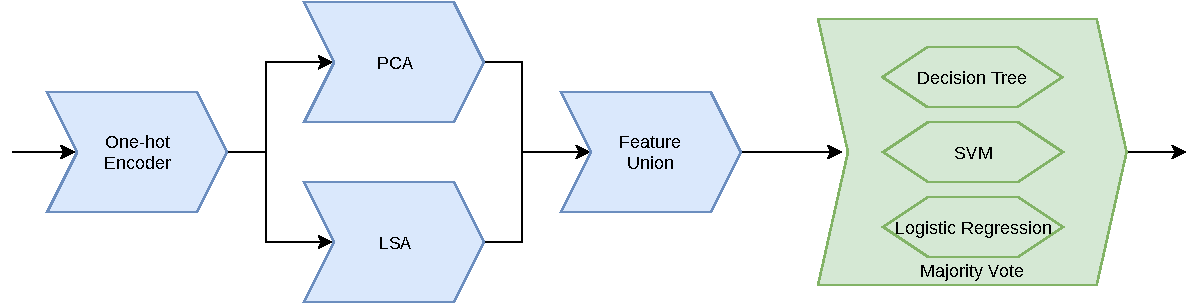
\includegraphics[width=\textwidth]{gfx/Figures/Theory/ComplexPipeline.pdf}
    \caption{Example for a more complex pipeline with four pre-processing components in blue: A One-hot Encoder, a Feature Union of a PCA and a LSA. The learning model in green is a Majority Voter as an aggregation of a Decision Tree, a SVM and a Logistic Regression Classifier. }
	\label{fig:theory:complexPipeline}
\end{figure}
Model Selection where the resulting pipelines can have this complexity needs to add a structural relationship between the pipeline components to the selected components.
Therewith, Model Selection can be written as simple formalization with two things:
\begin{itemize}
    \item For all possible components $C=\{c_1, ..., c_n\}$ a $C' \subseteq C$ of components that will be used to construct the pipeline.
    \item A binary relation $\prec$ over $C'$ that defines which component is a data input for another component to define an order of the components for the pipeline as well as aggregation of several components with one component. 
\end{itemize}
Nevertheless, to find a valid set $C' \subseteq C$ is not a trivial task.
For example, when an aggregator for multiple parallel pre-processing components is needed, a valid choice could be a Feature Union component but a Decision Tree component would be invalid for this pipeline position.
Therefore, if the pipelines shall be allowed to be more complex than for example a single pre-processing component and a single learning model, there is a big set of constraints for valid subsets of the candidate space of the Model selection $C$.

\subsection{Model Configuration}
\label{sec:theory:automl:configuration}
With the resulting component set after the Model Selection step selected its candidate $C'=\{c_1, ..., c_r\}$ the pipeline is not ready to be used yet.
Usually each component of $c_k \in C'$ has a set of hyperparameter and for each one a concrete value is needed.
Therewith, the candidate space for the Model Configuration step is dependent on the resulting candidate from the Model Selection step.
Each component $c_k$ has a set of hyperparameter $\Theta_k=\{ \theta_{k,1}, ..., \theta_{k,j} \}$ where each hyperparameter has a range where the value for this hyperparameter has to be chosen from.
Such a range can for example be a numeric set $\mathbb{N}$ or a custom set like for example $\{\textrm{true}, \textrm{false}\}$.\newline
When combining all ranges $\bigcup\limits_{i=1}^r \Theta_i$ a parametrization space with dimension $r$ is defined as the candidate space for the Model Configuration step, where configuration vectors can be drawn.
An example for a concrete parametrization drawn from a three dimensional parameter space is shown in figure~\ref{fig:theory:parameterSpace}
\begin{figure}[ht!]
    \centering
    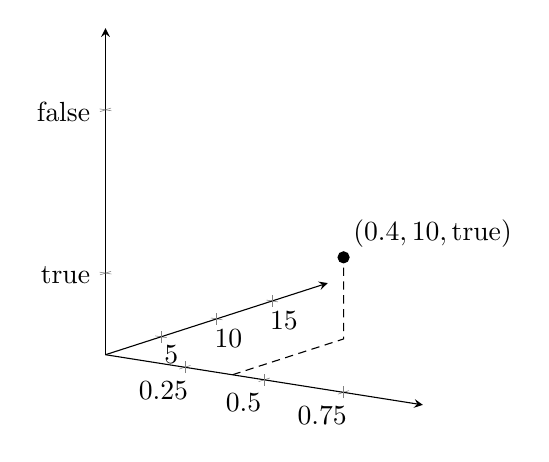
\begin{tikzpicture}
        \begin{axis}[
          view={35}{15},
          axis lines=center,
          xtick={0.25, 0.5, 0.75},ytick={5,10, 15},ztick={-10,-5,5,10},
          xmin=0,xmax=1,ymin=0,ymax=20,zmin=0.5,zmax=2.5,
          zticklabels={true, false},ztick={1,2},
          z tick label style={anchor=east}]
        ]
        \addplot3 [only marks] coordinates {(0.4,10,1)};
        \addplot3 [no marks,densely dashed] coordinates { (0.4,0,0.5) (0.4,10,0.5) (0.4,10,1)};
        \node [above right] at (axis cs:0.4,10,1) {$(0.4,10,\textrm{true})$};
        \end{axis}
    \end{tikzpicture}
    \caption{A parameter configuration with the values $(0.4,10,\textrm{true})$ inside the parameter space with the dimensions $[0..20]$, $[0, 1)$ and $\{\textrm{true}, \textrm{false}\}$ }
	\label{fig:theory:parameterSpace}
\end{figure}
Each of this vectors is a valid candidate and will result in a working pipeline instance created from $C'$ and configured with this vector.
When such a pipeline is constructed and configured with the vector values it can finally be evaluated as a candidate pipeline.

\subsection{Formalization of AutoML as an Optimization Problem}
\label{sec:theory:automl:optimization}
The choices in the Model Selection and Model Configuration step for one candidate out of the corresponding candidate spaces should not be arbitrary.
Evaluations of a candidate pipeline yield a score for this candidate and intuitively a suitable AutoML approach should try to select candidates with scores as good as possible.
Therefore, the AutoML problem is often considered as a special form of an optimization problem and can be formalized as one as well.\newline
\textcite{Feurer-Cash} give a formalization for AutoML problems as a so called \textit{Combined Algorithm Selection and Hyperparameter optimization} problem, or short \textit{CASH} problem.
Their definition is the following:
\begin{equation*}
    A^*, \lambda_* \in \> \underset{A^{(j)} \in \mathcal{A},\lambda \in \Lambda^{(j)}}{\mathrm{argmin}} \> \frac{1}{K} \sum_{i=0}^K \mathcal{L} (A_\lambda^{(j)}, D_{\textit{train}}^{(i)}, D_{\textit{valid}}^{(i)})
\end{equation*}
This formula consists out of the following parts:
\begin{itemize}
    \item $A^*$: The best solution of the algorithm selection, i.e. for the AutoML setting the best pipeline construction found in the Model Selection step
    \item $\lambda_*$: The best hyperparameter configuration for $A^*$ found in the hyperparameter optimization step, i.e. the Model Configuration step for AutoML
    \item $\mathcal{A}$: A set of possible algorithms to choose from and given in the form $\mathcal{A} = \{A^{1}, ..., A^{R} \}$, which is the set of all valid pipeline component combinations in the case of AutoML
    \item $\Lambda^{(j)}$: Each algorithm $A^{(j)} \in \mathcal{A}$ has a parameter configuration domain $\Lambda^{(j)}$, where a concrete parametrization $\lambda$ can be selected out of
    \item $\frac{1}{K} \sum_{i=0}^K $: This is used to calculate the K-fold cross-validation of a pipeline, but other evaluation metrics are also possible if the formula is adjusted accordingly
    \item $\mathcal{L} (A_\lambda^{(j)}, D_{\textit{train}}^{(i)}, D_{\textit{valid}}^{(i)})$: Is the loss, calculated with the loss function $\mathcal{L}$, of the algorithm $A^{(j)}$ configured with the parametrization $\lambda$, trained on the $i$-th split of the training data $D_{\textit{train}}^{(i)}$ and evaluated on the validation data $D_{\textit{valid}}^{(i)}$
\end{itemize}
In summary, the goal is to select an algorithm and a parameter configuration for this algorithm, such that the cross-validation loss for a for a given training and validation set is minimal.

\section{Black Box Optimization}
\label{sec:theory:optimization}
With the formalization of AutoML as a CASH problem the question arises if it can be tackled similar to standard textbook optimization problems, where established optimization algorithms exist.
Unfortunately, the CASH problem is a special case of optimization problem called \textit{Black Box} optimization problem.\newline
In the following will be explained in what way Black Box problems are different to the standard textbook optimization problem and why established optimization algorithms cannot be used.
Afterwards a selection of existing algorithms will be presented that can be used instead for the AutoML setting.
Finally, with the aid of the \textit{No-Free-Lunch Theorem}, it will be reasoned why these approaches cannot be optimal and why therefore a ensemble approach could be more promising.

\subsection{Differences to General Optimization Problems}
\label{sec:theory:optimization:differences}
\textcite{Boyd-Optimization} define a standard optimization problem as the following:
\begin{alignat*}{1}
    \underset{x}{\mathrm{minimize}} \textit{ or } \underset{x}{\mathrm{maximize}} \qquad & f_0(x)\\
    \textit{subject to} \qquad & f_i(x) \leq 0,\> i=1,...,m\\
                        &  h_j(x) \leq 0,\> j=1,...,p\\
\end{alignat*}
Here is the goal to find a value for the optimization variable $x$ such that $f_o(x)$ has either its minimum or maximum value.
Hereby, $x$ does not have to be a single value but can be a vector of values in the case of a multi-objective optimization problem.
$f_0$ is usually called a objective function or cost function.
The choices for $x$ can be limited by a set of inequality constraint functions $g_k$ and a set of equality constraint functions $h_i$.
If $m=p=0$, there are no constraint functions and the optimization problem is called unconstrained.
For such cases, x could be any value from the domain of $f_o$.\newline
If $f_0$ has certain properties, for example if it is convex, there are specialized optimization methods that can solve the optimization problem without the derivative $f_0'$.
But for general optimization algorithms, where no properties of $f_0$ besides derivability are expected, $f_0'$ is required to solve the optimization problem analytically.\newline
The problem is, for some optimization problems the exact formula of $f_0$ is not known or not given and therefore no derivative can be calculated such that the general optimization algorithms are not applicable.
Instead, it is only possible to obtain $f_0(x)$ for any requested $x$ for example by looking it up in a table or asking an expert.
For such problems it is only possible to observe the inputs and corresponding outputs of $f_0$ but the inner workings are hidden.
$f_0$ is metaphorically a black box, where something goes in and something comes out but it is not possible to look inside, and therefore such optimization problems are called Black Box optimization problems.\newline
AutoML, considered as a CASH problem, is a Black Box optimization problem as well.
It is not possible, or at least not yet realizable, to determine a general formula for $f_0$.
The relationship between the properties of the dataset, the different pipeline components with their configuration parameters and other factors, as for example randomness of some components, is way to complex and inscrutable to be formulated into a single cohesive function.
But it is possible to to get a evaluation of a $x$, i.e. a concrete pipeline with a complete configuration, by training and testing the pipeline with given data and a evaluation metric like for example a cross-validation.
The absence of a concrete formula for $f_0$ but the possibility to determine $f_0(x)$ renders AutoML as a Black Box optimization problem.\newline
Without the possibility to determine a optimal or near optimal candidate analytically, in the case of a Black Box optimization problem a series of candidates has to be selected and evaluated while trying to find or at least approximate a optimal solution.
Now the question remains for the AutoML setting how candidates from the two presumably large candidate spaces of Model Selection and Model Configuration should be selected for each iteration and how such a approximation can be attempted.\newline
A solely random selection in every iteration is not very likely to find good results with such a high number of choices.
Since the approach evaluates several candidates iteratively, a better approach would be to base the selection on knowledge gathered from previous iterations.\newline
Several algorithms were developed to tackle such a iteratively approximation of the optimum of a Black Box optimization problem.
Some of them have already showed promising results for AutoML CASH problems and therefore the current state-of-the-art AutoML research works primarily with the following three optimization strategies:
\begin{itemize}
    \item (Heuristic) Search
    \item Genetic and Evolutionary Algorithms
    \item Bayesian Optimization
\end{itemize}
In general is every Black Box optimization strategy defined by a selection of candidates out of the candidate space that will is evaluated and an order in which they are evaluated.
Hereby, the selection as well as the order can be defined in many ways.
For example it could be partially or fully pre-defined or random.
Also it could be defined implicitly and other selected candidates and their order can depend on the knowledge gathered from the evaluation of one candidate.\newline
For each one of the aforementioned Black-Box optimization strategies this candidate selection and candidate order will be explained in general and on the basis of some concrete algorithms, which were used in the AutoML research.
These explanations of the strategies will be supported with a simple running example.
The unconstrained target function $f_0(\begin{bmatrix}x\\y \end{bmatrix}) = x^2 + y^2$, which can be seen in figure~\ref{fig:theory:target-function}, shall be minimized.
This function is defined in $\mathbb{R}^2$ and has one global minimum.
\begin{figure}[ht!]
    \centering
    \begin{subfigure}{0.48\textwidth}
        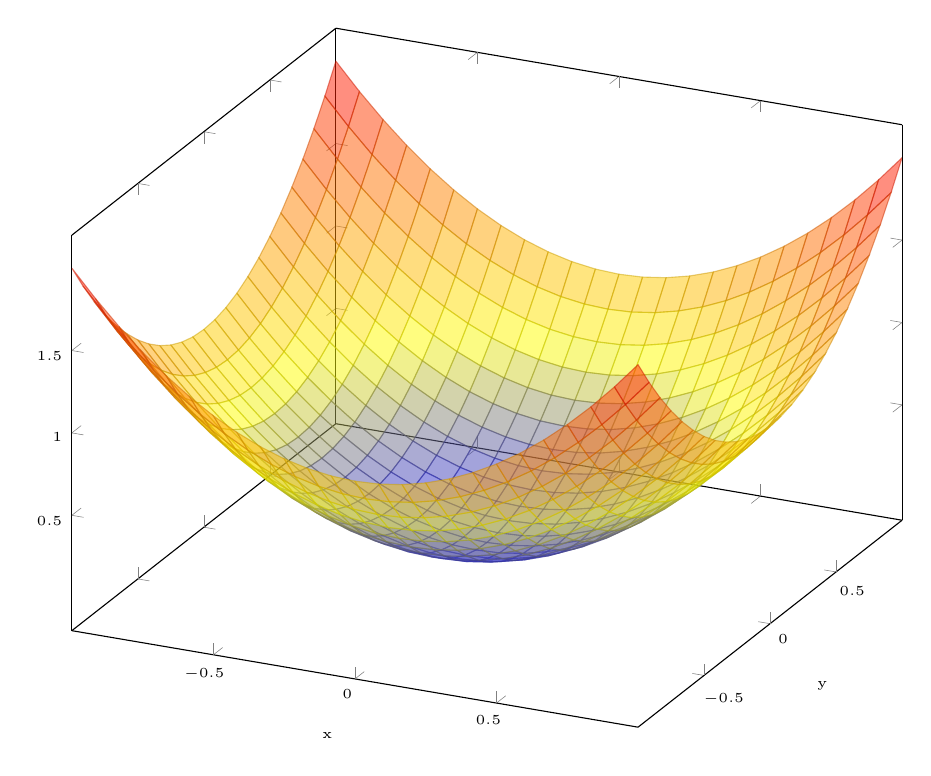
\begin{tikzpicture}
            \begin{axis}[
                xmin=-1,xmax=1,ymin=-1,ymax=1,
                width=\textwidth,
                xlabel = {x},
                ylabel = {y},
                xtick = {-0.5,0,0.5},
                ytick = {-0.5,0,0.5},
                ztick = {0.5,1,1.5},
                tick label style={font=\tiny},
                label style={font=\tiny}
            ]
                \addplot3[
                    surf,
                    opacity=0.5,
                    samples=25, samples y=25,
                    domain=-1:1, domain y=-1:1
                ]
                {x^2+y^2};
            \end{axis}
        \end{tikzpicture}
    \end{subfigure}
    \begin{subfigure}{0.48\textwidth}
        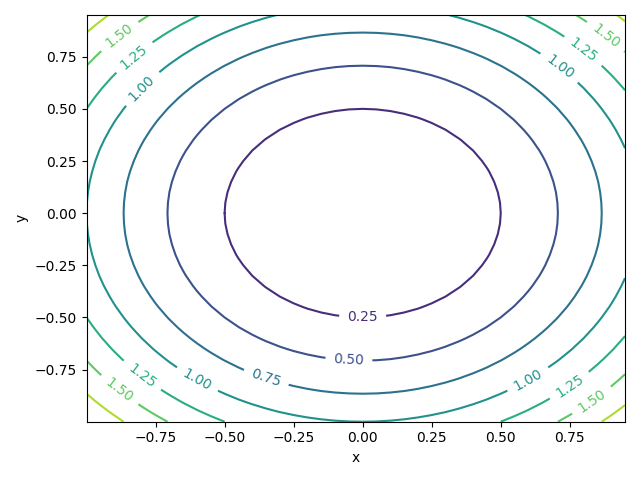
\includegraphics[width=\textwidth]{gfx/Figures/Theory/OptimizationTargetFunctionContour.png}
    \end{subfigure}
    \caption[.]{A two dimensional target function with a global minimum at \ensuremath{\begin{bmatrix} 0\\0 \end{bmatrix}}. On the right as a surface plot and on the left as a contour plot.}
    \label{fig:theory:target-function}
\end{figure}

\subsection{Optimization by Searching}
\label{sec:theory:optimization:search}
Optimizing with a search will evaluate candidates with the concept of \textit{Neighborhood} between candidates.
Starting with a single starting candidate, the search will extend its set of evaluated candidates by evaluating a neighboring candidate of one candidate out of this set.
The concrete definition of this neighborhood concept is depending of the examined search space, modelled out of the candidate space, and the applied search algorithm.
For example, a neighbor could be any candidate within a certain distance of another candidate or a graph could be created out of a set of candidates and neighbors of a candidate are the adjacent candidate nodes in the graph.
Which neighbor should be selected for evaluation next, therefore defining the order of candidate evaluations implicitly, can vary with the different approaches as well.
It could be completely random, pre-defined before the search starts or based on a heuristic scoring of the candidates.\newline
A wide range of search algorithms were developed in the corresponding research area and the most of them are applicable for optimization problems as well with a suitable neighborhood concept.
Some search algorithms are used in state-of the art AutoML approaches and three of them are explained in more detail with the aid of the running example in the following.\newline
\newline
\textbf{Random Search}: The Random Search Algorithm comes in two variants.
In the first one the candidates are completely drawn randomly out of the whole candidate space and evaluated.
When the optimization budget is spent, the best candidate is returned as the result.
Since this method does not use any knowledge gathered during the optimization, it depends on luck and the optimization budget if the optimal solution or at least a near optimal solution is found.\newline
In the second one, a starting candidate is drawn at random out of the candidate space and evaluated.
The next candidate will be randomly drawn out of a hypersphere with a pre-defined radius around the starting candidate and evaluated.
If the drawn candidate has a better evaluation score than the starting candidate, the next candidate will be drawn from a hypersphere around the second candidate and from the hypersphere of the starting candidate otherwise.
This loop is continued until the optimization budget is spent. Since this method is very prone to local minima/maxima, it is a possible improvement to remember the current best candidate, select a new completely random start point and start the loop over, if there was no improvement in the last $n$ iterations of the current loop.
Both variants are illustrated for the running example in figure~\ref{fig:theory:random-search}.\newline
One example of the Random Search algorithm applied in the context of AutoML is the \textit{Hyperband} approach~\cite{Li-Hyperband}.
Here, multiple parallel working instances of Random Searches are evaluating candidates in a joint space of Model Selection and Model Configuration to cover as much of the candidate space as possible.
The initial problem is that multiple instances combined require a big portion of the optimization budget.
This was tackled by treating each random search as the arm of the bandit and canceling single search instances over time that do not find candidates with high evaluation scores and which therefore probably have a low regret.
By terminating some probably low performing searches the optimization budget can be spent on mor promising search instances.
Strategies like this are often referred to as \textit{Early Stopping}.
In the context of Hyperband, selecting the search instances which will not be stopped early is done in a non-stochastic manner with the \textit{Successive Halving} algorithm~\cite{Jamieson-SuccessiveHalving}.
\begin{figure}[ht!]
    \centering
    \begin{subfigure}{0.48\textwidth}
        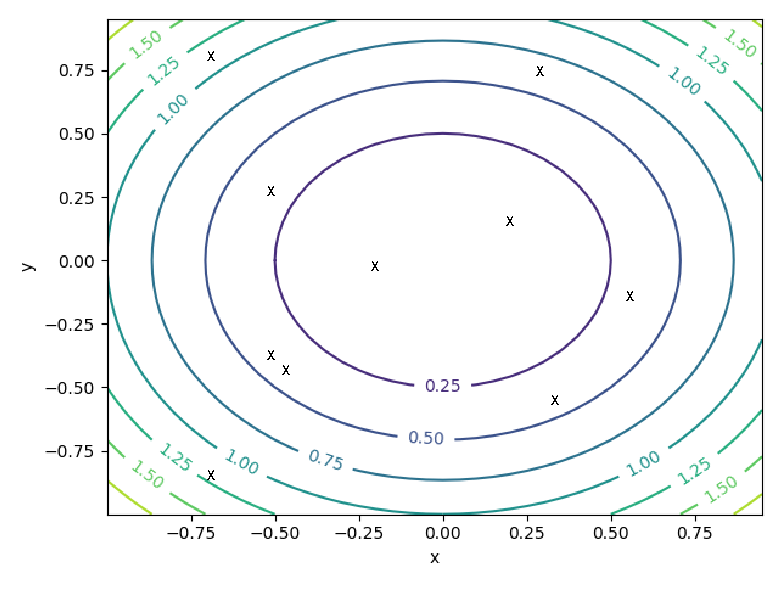
\includegraphics[width=\textwidth]{gfx/Figures/Theory/RandomSearch.pdf}
    \end{subfigure}
    \begin{subfigure}{0.48\textwidth}
        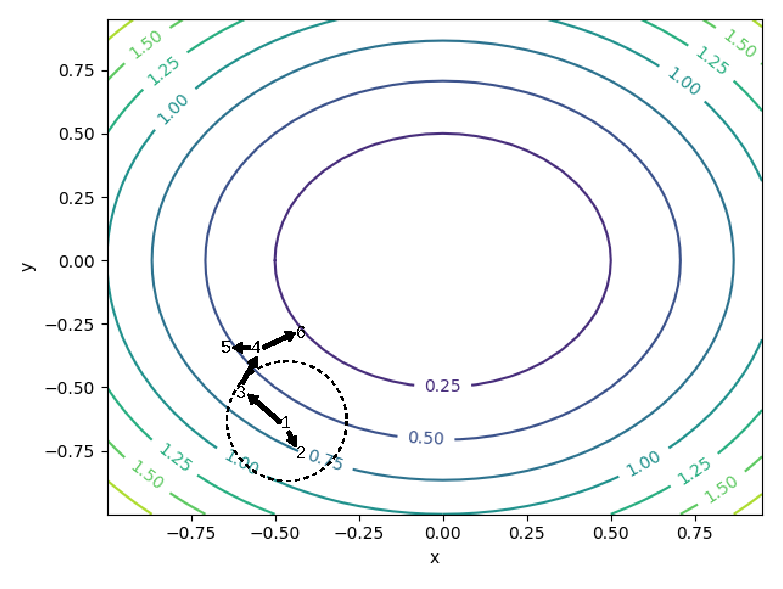
\includegraphics[width=\textwidth]{gfx/Figures/Theory/RandomSearchHypersphere.pdf}
    \end{subfigure}
    \caption{On the left is the first variant with a few randomly selected candidates. On the right are six possible first iterations of the second variant. The hypersphere is only shown for the first candidate.}
    \label{fig:theory:random-search}
\end{figure}
\newline

\textbf{Grid Search}: A Grid Search tries to cover with a na\"ive brute-force approach as much of the candidate space as possible.
From each dimension of the candidate space a few values are selected either manual, or more commonly by selecting values from the dimensions allowed range in periodic intervals.
For example, if the x-dimension of the running example should be evaluated in the range $[-1,1]$, depending on the available optimization, potential value selections for this dimension could be $\{-1,0,1\}$ or $\{-0.75,-0.25,0.25,0.75\}$.\newline
After selecting the value sets for each dimension, the Cartesian product of all sets is calculated.
The elements of this Cartesian product, which are valid candidates because they have a value of each dimension, are the candidates that will be evaluated during the search and for the order of evaluations any arbitrary sequence of the sets elements can be selected.
After either all candidates from the Cartesian product are evaluated or if the optimization budget is spent, the best evaluated candidate is the overall optimization result.
An illustration of a Grid Search over the candidate space of the running example can be seen in figure~\ref{fig:theory:grid-search}.\newline
Therefore, as opposed to Random Searches where by chance only a small portion of the candidate space could be covered, a certain coverage of the space is assured.
Especially in contrast to the second variant of the Random Search, the advantage is that there is no risk of getting stuck in a local optimum.
But im comparison of with the second Random Search variant the main drawback of a Grid Search comes clear, i.e. a Grid Search does not utilize the knowledge gathered from previous evaluations at all, since the evaluation order is completely predefined.
This, even if the Grid Search would evaluate a candidate comparably close to a global optimum, it would completely disregard this chance and not continue the search closely to this candidate to potentially find this global optimum.\newline
Grid Searches are as well as Random Searches classical algorithm choices for Hyperparameter optimization because they are easy to implement and very resource-efficient due to their simplicity such that a high number of candidate evaluation can be performed.
In the context of AutoML, a 2-dimensional Grid Search was utilized in the Weka toolbox~\cite{Witten-Weka} for a simple AutoML approach.
There, a joint candidate space was searched with a set of classifiers for model selection on one dimension and the other dimension is used to select the amount of components of Partial Least Squares filter, which is used as a pre-processor, and can therefore be considered as a simple model configuration.
\begin{figure}[ht!]
    \centering
    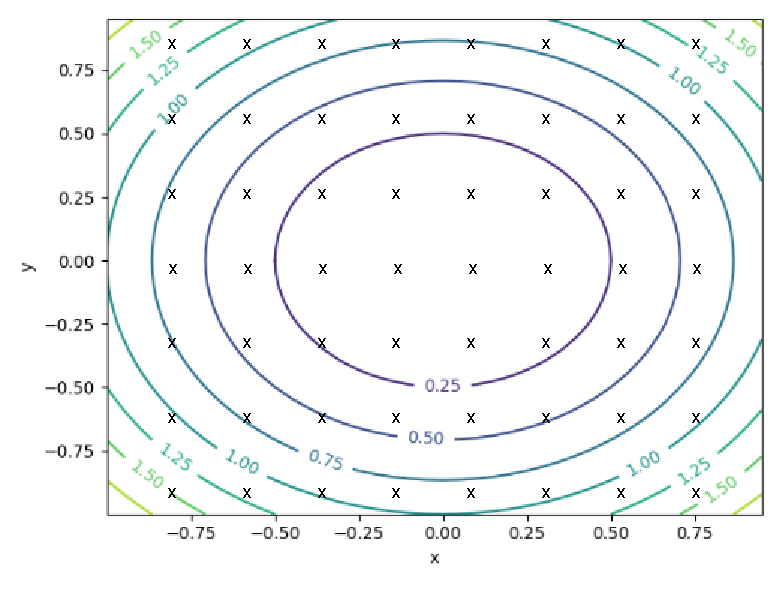
\includegraphics[width=\textwidth]{gfx/Figures/Theory/GridSearch.pdf}
    \caption{Illustration of a Grid Search covering the search space of the running example systematically.}
    \label{fig:theory:grid-search}
\end{figure}
\newline

\textbf{(Heuristic) Graph Search}: While a Random Search does it partially leaf to chances which candidates are evaluated, the candidate space will not be adequately covered with a high probability, a Grid Search will have certain coverage guarantees by default.
On the other hand, a Grid Search will not utilize any gathered knowledge about the candidate space while at least the second variant of a Random Search is capable of utilizing knowledge about one prior evaluation.
A Graph Search, usually in combination with a heuristic for search guidance, tries to achieve a trade-off between the advantages of both other presented search algorithms, i.e. having a solid coverage of the candidate space as well as utilizing knowledge gathered during the search.

\subsection{Genetic and Evolutionary Optimization}
\label{sec:theory:optimization:genetic}

\Blindtext

\subsection{Bayesian Optimization}
\label{sec:theory:optimization:bayesian}

\Blindtext

\subsection{No-Free-Lunch Theorem}
\label{sec:theory:optimization:lunch}

\Blindtext

\section{Related Work}
\label{sec:theory:related}

\Blindtext
